\documentclass[10pt,twocolumn,letterpaper]{article}

\usepackage{cvpr}
\usepackage{times}
\usepackage{epsfig}
\usepackage{graphicx}
\usepackage{amsmath}
\usepackage{amssymb}
\usepackage{subcaption}
\usepackage{booktabs}
\usepackage{algorithm}
\usepackage{algpseudocode}
\usepackage{listings}
\usepackage{xcolor}
\usepackage{url}

% Include hyperref last
\usepackage[pagebackref=true,breaklinks=true,letterpaper=true,colorlinks,bookmarks=false]{hyperref}

\cvprfinalcopy % Uncomment for camera-ready version

\def\cvprPaperID{****}
\def\httilde{\mbox{\tt\raisebox{-.5ex}{\symbol{126}}}}

\ifcvprfinal\pagestyle{empty}\fi

% Figures are generated by scripts/plot_results.py into ../figures
\graphicspath{{../figures/}{./}}

\lstset{
  language=C++,
  basicstyle=\ttfamily\scriptsize,
  keywordstyle=\color{blue!60!black}\bfseries,
  commentstyle=\color{green!40!black},
  columns=fullflexible,
  frame=single,
  framerule=0.3pt,
  breaklines=true,
  showstringspaces=false
}

% Less restrictive float placement: avoids pushing all figures to the end
\renewcommand{\topfraction}{0.9}
\renewcommand{\bottomfraction}{0.8}
\renewcommand{\textfraction}{0.1}
\renewcommand{\floatpagefraction}{0.8}
\renewcommand{\dbltopfraction}{0.9}
\renewcommand{\dblfloatpagefraction}{0.8}
\setcounter{topnumber}{3}
\setcounter{dbltopnumber}{2}

\newcommand{\x}{\ensuremath{\times}}

\begin{document}

%%%%%%%%% TITLE
\title{Parallel Programming for Machine Learning \\ Final-term assignment: \textit{Mean shift clustering}}

\author{Francesco Acciaioli\\
University of Florence\\
{\tt\small francesco.acciaioli@stud.unifi.it}
}

\maketitle
\thispagestyle{empty}

%%%%%%%%% ABSTRACT
\begin{abstract}
Mean shift is a non-parametric clustering algorithm that finds the modes of a kernel density
estimate; applied to the colours of an image it produces a segmentation without fixing the number
of clusters in advance. Its cost is $O(N^2)$ per iteration in the number of pixels $N$, which makes
the sequential version slow even on small images. This report presents a C++17 implementation in
four variants: a scalar sequential baseline, a single-thread SIMD version, an OpenMP parallel
version with a vectorized inner loop, and an Array-of-Structures variant used to study the memory
layout. The parallelization exploits the independence of the points: no synchronization is needed
except for reductions. Experiments on images of the Berkeley Segmentation Dataset (BSDS500), run on
an Apple M2 (4 performance + 4 efficiency cores, 128-bit NEON), show a $1.84\x$ gain from
vectorization alone and a total speedup of $8.7\x$ with 8 threads on a $128\x128$ image
(13.15\,s $\rightarrow$ 1.51\,s), reaching $15.2\x$ for large bandwidths. Thread scaling is almost
linear up to the 4 performance cores and then limited by the slower efficiency cores.
\end{abstract}

%%%%%%%%% BODY TEXT
\noindent\large\textbf{Future Distribution Permission}\\
\indent The author(s) of this report give permission for this document to be distributed to Unifi-affiliated students taking future courses.

\section{Introduction}

This report presents the implementation and performance analysis of a sequential and a parallel
version of the \textit{mean shift} clustering algorithm, applied to colour image segmentation. The
source code, the benchmark harness and all the results are available in the public repository
\url{https://github.com/FranciAccia/MeanShiftParallel}.

\subsection{Problem description and motivation}
Mean shift~\cite{fukunaga1975,cheng1995,comaniciu2002} is a non-parametric iterative procedure
that locates the local maxima (\emph{modes}) of a probability density estimated from the data with
a kernel density estimate (KDE). Every data point is moved uphill along the gradient of the density
until it converges to a mode; points that reach the same mode form a cluster. Unlike K-means, the
number of clusters is not specified in advance: the only parameter is the \emph{bandwidth} $h$ of
the kernel, which sets the scale of the structures that are considered distinct
(Figure~\ref{fig:kde}).

In image segmentation each pixel is a point in the RGB colour space. After convergence each pixel
is replaced by the colour of its mode, which produces a flat-colour segmentation of the image
(Figure~\ref{fig:segmentations}).

\begin{figure}[!htb]
    \centering
    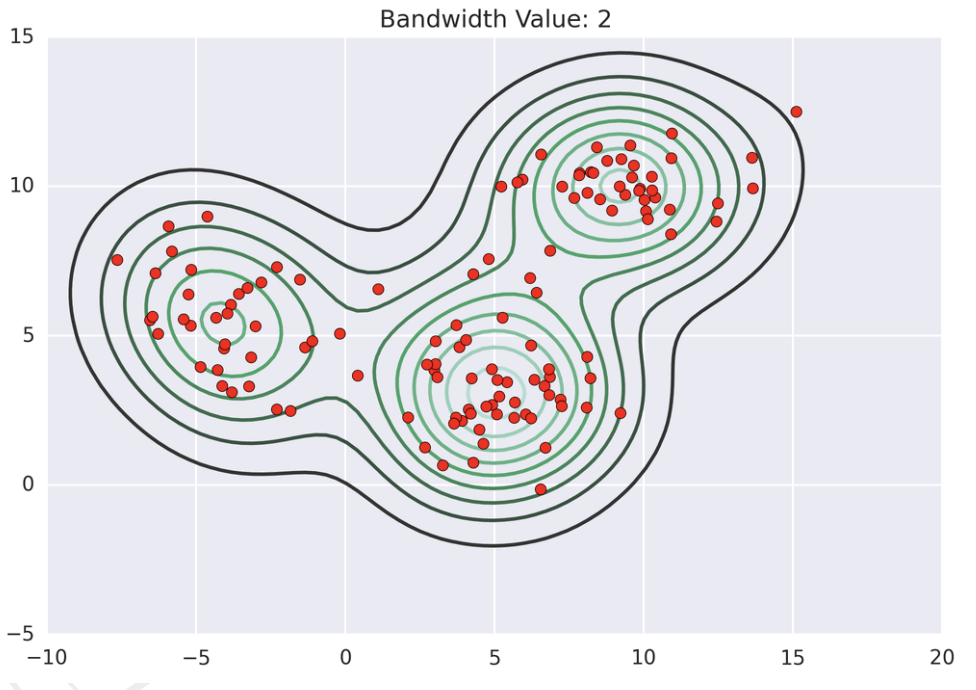
\includegraphics[width=0.85\linewidth]{kde_example.png}
    \caption{Kernel density estimate of a 2D point set: the modes of the density (centres of the
    contour lines) are the cluster centres found by mean shift.}
    \label{fig:kde}
\end{figure}

\begin{figure*}[!t]
    \centering
    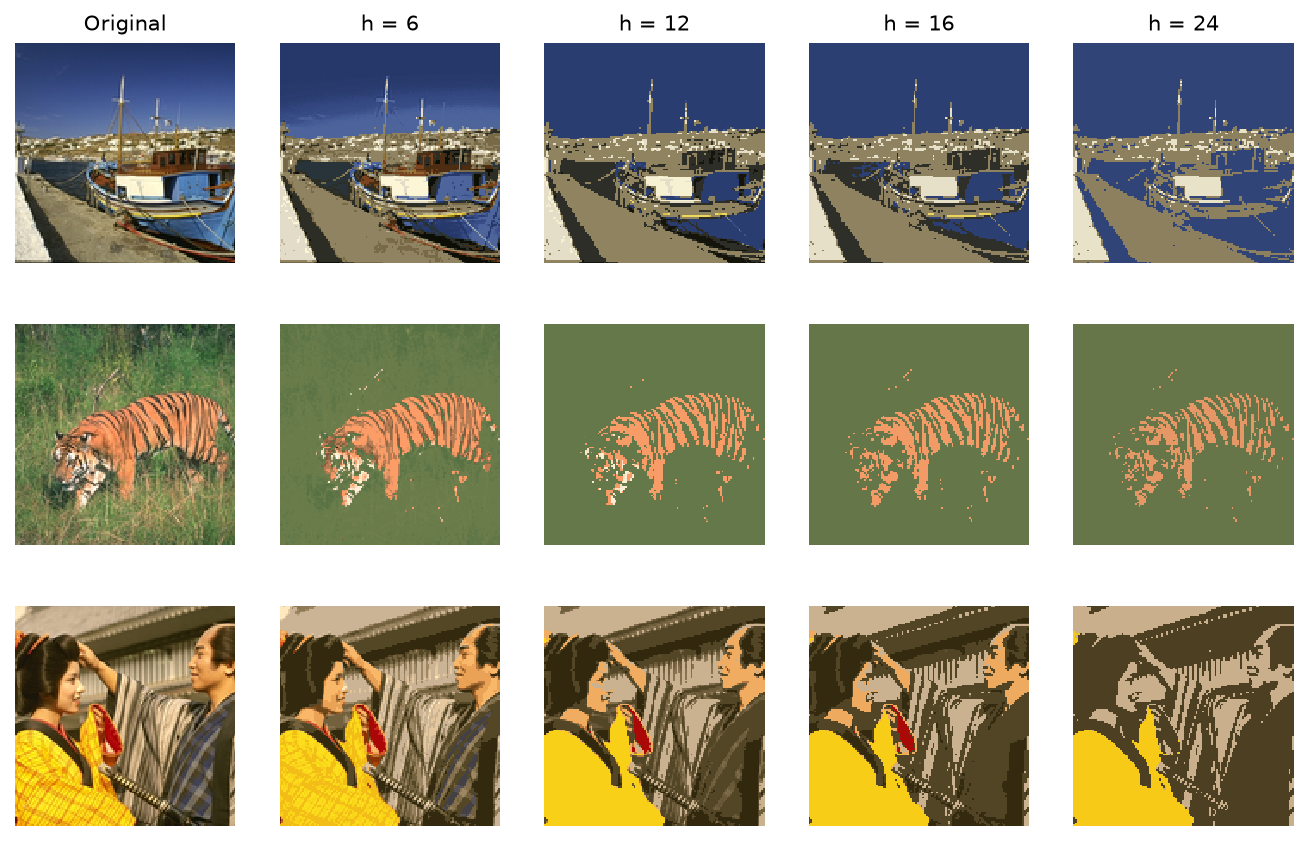
\includegraphics[width=0.82\textwidth]{segmentations.png}
    \caption{Segmentation of the three BSDS500 images ($128\x128$) for increasing bandwidth. A small
    $h$ keeps many shades (over-segmentation), a large $h$ merges distinct objects.}
    \label{fig:segmentations}
\end{figure*}

\subsection{Computational challenges}
For $N$ points, every iteration of every point has to evaluate the kernel against all the $N$
points of the dataset, so the cost is $O(N^2)$ per iteration, multiplied by the number of
iterations needed to converge (about 43 per point in our main configuration). A $128\x128$ image
($N = 16\,384$) already requires $\approx 1.1\cdot 10^{10}$ kernel evaluations, which take
13\,s on one core. A full-resolution BSDS image ($481\x321$) would take hours.

The problem is however \emph{embarrassingly parallel}: the trajectory of each point depends only
on the original dataset, which is read-only, and not on the other trajectories.

\subsection{Objectives}
\begin{enumerate}
    \item A sequential, scalar baseline in C++ used as reference for correctness and time.
    \item A parallel version that combines OpenMP multi-threading over the points with SIMD
    vectorization of the inner loop over the neighbours.
    \item An experimental analysis of speedup, efficiency and scalability, and of the effect of the
    bandwidth, of the OpenMP scheduling policy and of the memory layout (AoS vs SoA).
\end{enumerate}

\section{Algorithm description}

\subsection{Sequential algorithm}
Let $x_1,\dots,x_N \in \mathbb{R}^3$ be the RGB colours of the pixels (values in $[0,255]$). With a
Gaussian kernel of bandwidth $h$, each point $y$ is updated with the weighted mean of the dataset:
\begin{equation}
    y \leftarrow \frac{\sum_{j} w_j\, x_j}{\sum_j w_j}, \qquad
    w_j = \exp\!\left(-\frac{\|y - x_j\|^2}{2h^2}\right).
    \label{eq:shift}
\end{equation}
This is the \emph{full} mean shift (not the blurring variant): the points $x_j$ never change, only
the copy $y$ of each point moves. Weights beyond $3h$ are negligible ($w < 0.012$) and are treated
as zero. A point stops when the shift is smaller than $\varepsilon h$ with $\varepsilon = 10^{-3}$,
or after 100 iterations. The complete algorithm has three phases:
\begin{enumerate}
    \item \textbf{Shift} (Algorithm~\ref{alg:ms}): every point converges to its mode,
    $O(N^2 \cdot \text{iter})$.
    \item \textbf{Mode detection}: modes are scanned in index order; a mode becomes a new cluster
    centre if it is farther than $h/2$ from all the centres found so far, $O(N K)$ with $K$
    clusters.
    \item \textbf{Labelling}: each pixel is assigned to the centre nearest to its mode, $O(N K)$.
\end{enumerate}
Phases 2 and 3 take about 0.2\,ms against 7--13\,s of phase 1 (0.01\%), so all the optimization
effort is spent on phase 1.

\begin{algorithm}[!htb]
\caption{Shift phase of mean shift}
\label{alg:ms}
\begin{algorithmic}[1]
\For{$i = 1 \dots N$} \Comment{independent points}
  \State $y \gets x_i$
  \Repeat
    \State $s \gets 0,\; s_w \gets 0$
    \For{$j = 1 \dots N$} \Comment{all the neighbours}
      \State $d^2 \gets \|y - x_j\|^2$
      \If{$d^2 \le (3h)^2$}
        \State $w \gets \exp(-d^2 / 2h^2)$
        \State $s \gets s + w\,x_j$;\; $s_w \gets s_w + w$
      \EndIf
    \EndFor
    \State $y_{old} \gets y$;\; $y \gets s / s_w$
  \Until{$\|y - y_{old}\| < \varepsilon h$ \textbf{or} 100 iterations}
  \State $mode_i \gets y$
\EndFor
\end{algorithmic}
\end{algorithm}

\subsection{Parallelizable sections}
\begin{itemize}
    \item \textbf{Outer loop over the points} (coarse grain): each point reads only the original
    dataset and writes only its own mode, so the iterations are independent and can be distributed
    among threads. The number of iterations to convergence varies from point to point, so the work
    is not uniform and the scheduling policy matters.
    \item \textbf{Inner loop over the neighbours} (fine grain): the same arithmetic is applied to
    all the $N$ points and the results are accumulated in four sums ($s_r, s_g, s_b, s_w$), a
    reduction that can be vectorized.
    \item \textbf{Labelling} is also independent per pixel and is parallelized, while mode
    detection is kept sequential so that the clusters do not depend on the number of threads.
\end{itemize}

\section{Parallel implementation}

\subsection{Variants}
All the variants share the same algorithm, parameters and kernel and differ only in how phase 1 is
executed (Table~\ref{tab:variants}).

\begin{table}[h]
\centering
\small
\begin{tabular}{@{}lll@{}}
\toprule
\textbf{Variant} & \textbf{Parallelism} & \textbf{Layout} \\ \midrule
\texttt{seq}     & none, scalar (baseline)           & AoS \\
\texttt{simd}    & 1 thread, \texttt{omp simd} inner loop & SoA \\
\texttt{par}     & \texttt{omp parallel for} + SIMD  & SoA \\
\texttt{par\_aos} & as \texttt{par} (layout study)   & AoS \\ \bottomrule
\end{tabular}
\caption{Implemented variants.}
\label{tab:variants}
\end{table}

\subsection{Thread-level parallelism (OpenMP)}
The outer loop over the points is distributed among the threads with a single directive:
\begin{lstlisting}
#pragma omp parallel for \
        schedule(runtime) reduction(+ : total)
for (int i = 0; i < n; ++i) {
    Pixel y = d.aos[i];
    total += converge_simd_soa(R, G, B, n, y,
                               k, max_iter);
    modes[i] = y;
}
\end{lstlisting}
\texttt{schedule(runtime)} lets the benchmark choose the policy (static, dynamic, guided and the
chunk size) through \texttt{omp\_set\_schedule} without recompiling. Unless stated otherwise,
\texttt{dynamic,16} is used (Section~\ref{sec:schedule}).

\subsection{Synchronization}
No locks, \texttt{critical} sections or atomics are needed: the dataset is only read, and the
iteration $i$ writes only \texttt{modes[i]}, once, at the end of its convergence. The only shared
quantity is the total number of iterations (used for statistics), which is accumulated with
\texttt{reduction(+:total)}, so each thread keeps a private counter merged at the end of the loop.
False sharing on \texttt{modes} is possible only at chunk boundaries and happens once per point
after $\approx 43 \cdot N$ kernel evaluations, so it is negligible and no padding was added.

\subsection{Vectorization (SIMD)}
The inner loop is vectorized with \texttt{\#pragma omp simd reduction(+:sr,sg,sb,sw)}. On the
ARM NEON unit of the M2 (128-bit registers) this processes 4 single-precision neighbours per
instruction. Two changes were needed to make the loop vectorizable:
\begin{itemize}
    \item \textbf{Branchless cutoff.} The \texttt{if} on the $3h$ cutoff becomes a select,
    \texttt{w = (d2 <= cutoff2) ? exp(...) : 0}, so all lanes execute the same instructions.
    \item \textbf{Inline exponential.} \texttt{std::exp} inside the loop is compiled into a call
    per lane, which cancelled the SIMD gain. It was replaced by \texttt{fast\_exp}, an inline,
    branchless approximation ($2^k$ written in the IEEE-754 exponent times a degree-5 polynomial,
    relative error $< 4\cdot10^{-7}$). To make the comparison fair, the scalar baseline uses the same
    function, so \texttt{seq} vs \texttt{simd} measures only the effect of vectorization.
\end{itemize}
The baseline instead keeps the branch, which lets it skip the exponential for the points beyond the
cutoff, and its vectorization is explicitly disabled
(\texttt{\#pragma clang loop vectorize(disable)}). The clang vectorization report
(\texttt{-Rpass=loop-vectorize}) confirms that the inner loops of \texttt{simd}/\texttt{par} and
\texttt{par\_aos} are vectorized with width 4 and interleave count 2, and that the loop of
\texttt{seq} is not. No \texttt{-ffast-math} is used: floating-point sums are reordered only where
\texttt{omp simd reduction} explicitly allows it.

\subsection{Data layout}
The \texttt{Dataset} keeps the pixels in both layouts, built once when the image is loaded (outside
the timed region): an Array of Structures (\texttt{struct Pixel \{float r,g,b;\}}) and a Structure of
Arrays (three contiguous arrays \texttt{r}, \texttt{g}, \texttt{b}). With SoA, 4 consecutive values
of the same channel are loaded with one vector load; with AoS the loop accesses memory with stride 3
and the channels have to be de-interleaved. Single precision is enough for colours in $[0,255]$ and
doubles the number of SIMD lanes compared to \texttt{double}.

\subsection{Difficulties}
\begin{itemize}
    \item The first SIMD version used \texttt{std::exp} and was not faster than the scalar code;
    the inline exponential solved it.
    \item Non-uniform work (points in textured regions need more iterations than points in
    uniform regions) made the default static schedule the slowest (Section~\ref{sec:schedule}).
    \item The test machine has no fan: under continuous load the times grew by up to 50\%, which
    required a cool-down between runs (Section~\ref{sec:setup}).
\end{itemize}

\begin{figure*}[!t]
    \centering
    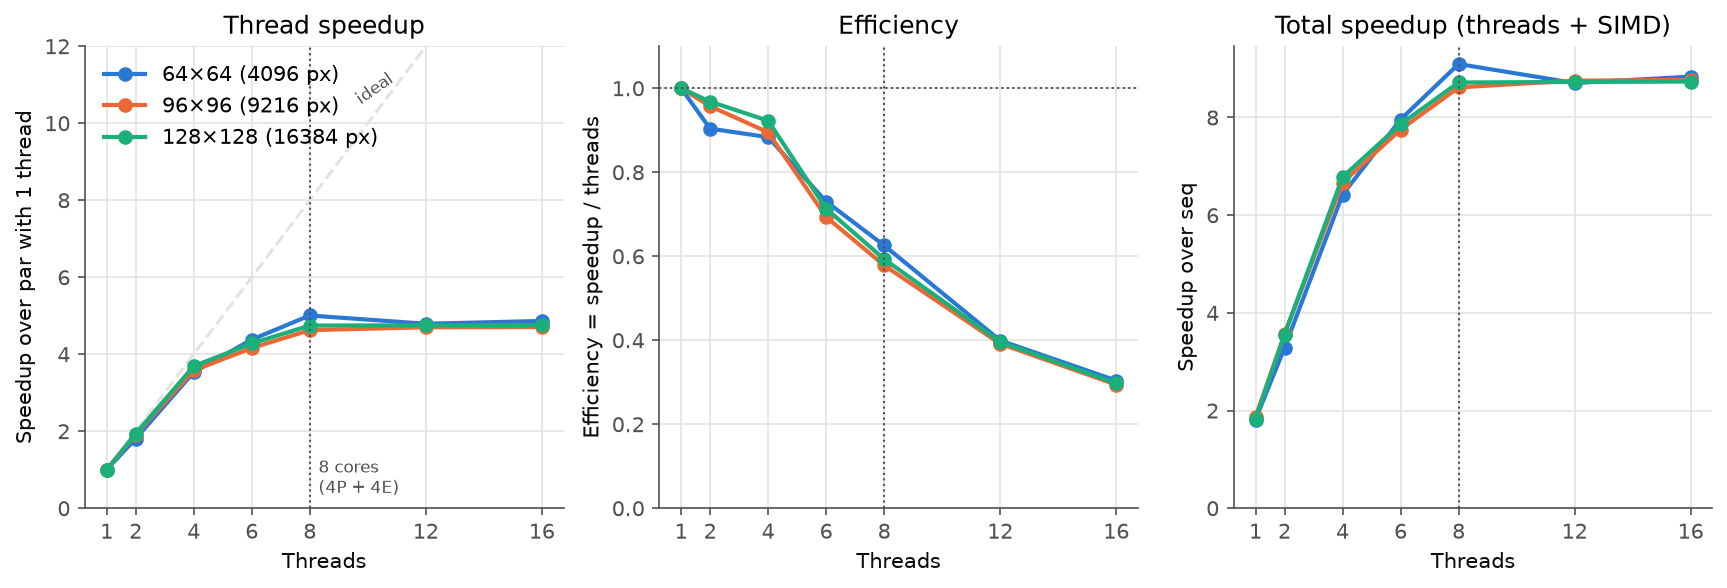
\includegraphics[width=\textwidth]{scaling.png}
    \caption{Strong scaling for the three image sizes. Left: speedup of the threads over
    \texttt{par} with 1 thread (dashed line: ideal). Centre: efficiency. Right: total speedup over
    the scalar sequential baseline. The dotted line marks the 8 cores of the M2.}
    \label{fig:scaling}
\end{figure*}

\section{Experimental setup}
\label{sec:setup}

\subsection{Hardware and software}
\begin{itemize}
    \item \textbf{CPU}: Apple M2 (MacBook Air, Mac14,2), 8 cores: 4 performance (P, up to
    3.5\,GHz, 128\,KB L1d each, 16\,MB shared L2) and 4 efficiency (E, up to 2.4\,GHz, 4\,MB shared
    L2); 128-bit ARM NEON SIMD; 8\,GB unified memory. Passive cooling (no fan).
    \item \textbf{Software}: macOS 26.6, Apple clang 21.0.0, LLVM OpenMP runtime (\texttt{libomp})
    21.1.8 from Homebrew, CMake 4.2.
    \item \textbf{Flags}: \texttt{-std=c++17 -O3 -march=native -Xpreprocessor -fopenmp}
    (Release build).
\end{itemize}

\subsection{Dataset and preprocessing}
Three real images from the BSDS500 test set~\cite{arbelaez2011} were chosen for their variety of
colours: 118015 (boats in a harbour, main image), 108004 (a tiger in the grass) and 145059 (people
in coloured clothes). A Python script crops the central square of each image and resizes it to
$64^2$, $96^2$ and $128^2$ pixels with a Lanczos filter. Resizing is necessary because of the
$O(N^2)$ cost; the $128^2$ size is the smallest one with a sequential time above 10\,s (13.15\,s at
$h=12$). Preprocessing is done once, offline, and is not part of the measurements; images are read
with \texttt{stb\_image}~\cite{stb}.

\subsection{Parameters}
The main configuration is image 118015, $128\x128$ ($N = 16\,384$), $h = 12$, 8 threads,
\texttt{dynamic,16}. The experiments vary one parameter at a time:
\begin{itemize}
    \item \textbf{Strong scaling}: 1, 2, 4, 6, 8, 12, 16 threads (up to $2\x$ the cores), on the
    three sizes.
    \item \textbf{Bandwidth}: $h \in \{6, 8, 12, 16, 24, 32\}$ ($96\x96$ to keep the sequential runs
    short).
    \item \textbf{Scheduling}: \texttt{static}, \texttt{static,1}, \texttt{static,64},
    \texttt{dynamic} with chunk 1, 16, 256, \texttt{guided}.
    \item \textbf{Layout}: AoS vs SoA with 1 and 8 threads.
\end{itemize}

\subsection{Methodology}
Each configuration runs 1 discarded warm-up and 5 measured runs; the report gives mean, standard
deviation, minimum, maximum and a 95\% confidence interval ($1.96\,\sigma/\sqrt{5}$). Wall-clock
time is measured with \texttt{omp\_get\_wtime()} around the clustering only (image loading and
layout conversion are excluded); CPU time (sum over all threads, user + system) is read with
\texttt{getrusage}. Speedup is $S(p) = T_{seq}/T_{par}(p)$ and efficiency $E(p) = S(p)/p$.

Because the machine is fanless, after each run the benchmark sleeps for as long as the run lasted
(at most 5\,s), so that every run starts from a similar temperature. macOS does not allow disabling
frequency scaling or pinning threads to cores. Background applications were closed during the
measurements.

\begin{figure*}[!t]
    \centering
    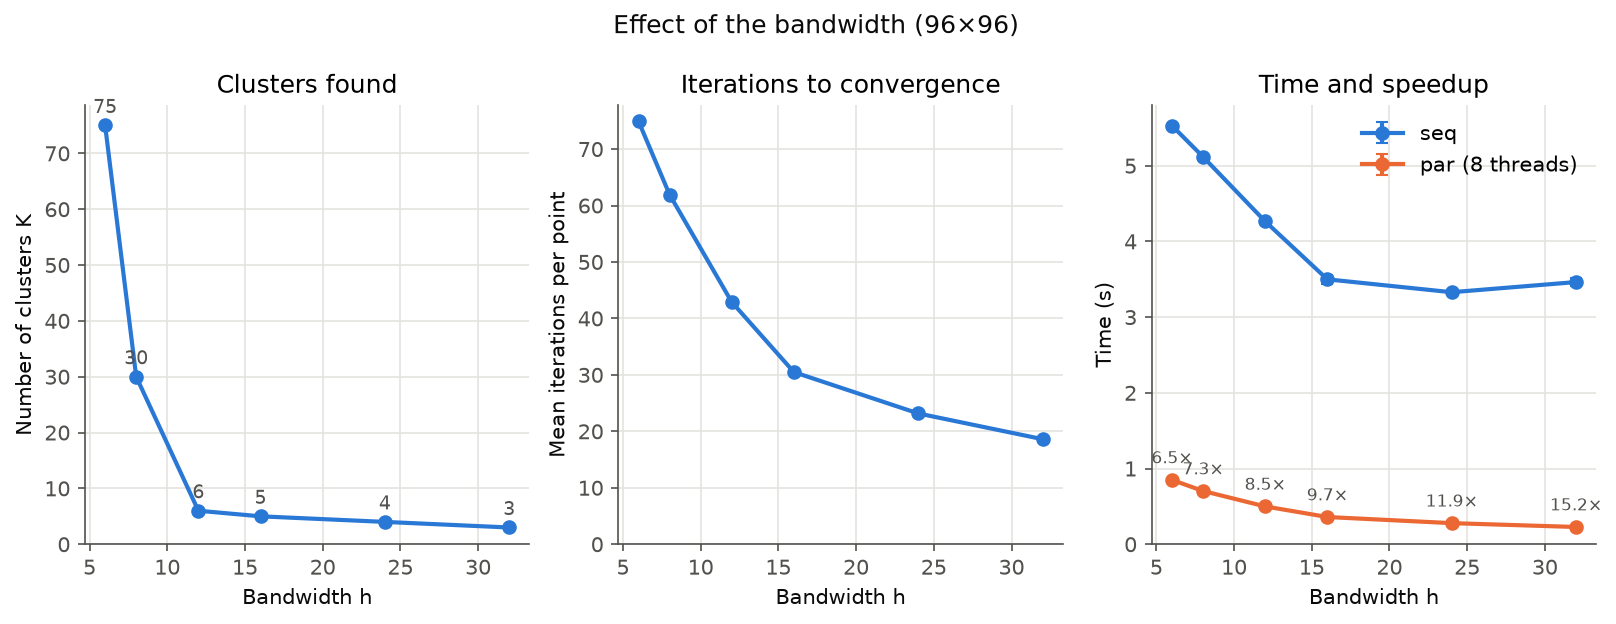
\includegraphics[width=0.9\textwidth]{bandwidth.png}
    \caption{Effect of the bandwidth on the $96\x96$ image: number of clusters, mean iterations per
    point, and time of \texttt{seq} and \texttt{par} (8 threads) with the resulting speedup.}
    \label{fig:bandwidth}
\end{figure*}

\section{Results and analysis}

\subsection{Correctness validation}
Before every benchmark, an automatic check runs all the variants on the three $64\x64$ images and
compares them with \texttt{seq}; the benchmark aborts if the check fails. The check requires the
same number of clusters, the same label for every pixel, and modes within 1\% of $h$ (0.12 on the
0--255 scale). The result is:
\begin{itemize}
    \item clusters and labels are identical for all variants (9/9, 5/5, 14/14 clusters,
    4096/4096 labels);
    \item the modes differ by at most $1.1\cdot10^{-2}$, $6.7\cdot10^{-2}$ and $7.5\cdot10^{-2}$.
\end{itemize}
The small differences are expected: the SIMD reduction sums in a different order, and the
stopping rule ($\varepsilon h$) lets two trajectories stop at slightly different points. The
\texttt{simd}, \texttt{par} and \texttt{par\_aos} variants produce exactly the same modes for any
number of threads, because each point is still computed by a single thread in the same order.

\subsection{Effect of vectorization}
Figure~\ref{fig:vectorization} compares \texttt{seq} and \texttt{simd} on one thread. The gain is
$1.83$--$1.86\x$ and does not depend on the image size. It is lower than the theoretical $4\x$ of
4-lane NEON because the two variants do different work: the scalar code skips the exponential for
every neighbour beyond $3h$, while the vector code computes it for all the neighbours and then
discards it with the select. Section~\ref{sec:bandwidth} confirms this.

\begin{figure}[!htb]
    \centering
    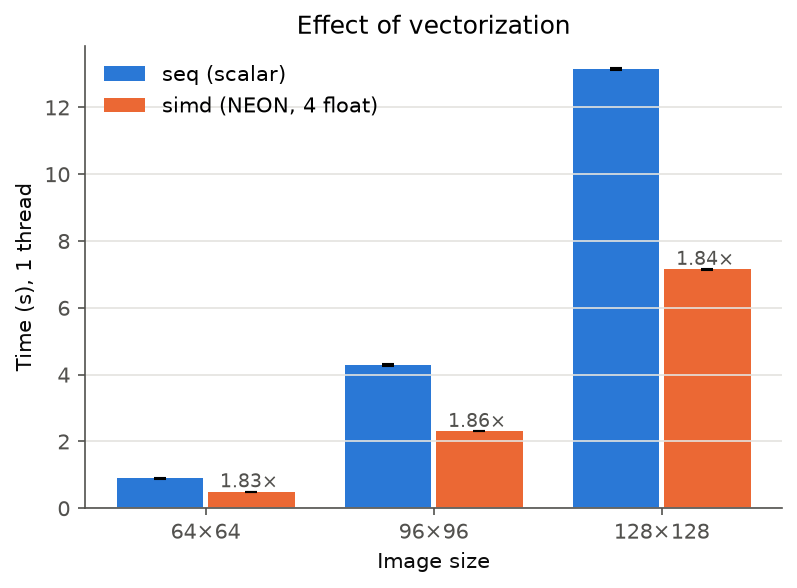
\includegraphics[width=\linewidth]{vectorization.png}
    \caption{Scalar baseline vs SIMD on a single thread, with 95\% confidence intervals and
    speedup of \texttt{simd} over \texttt{seq}.}
    \label{fig:vectorization}
\end{figure}

\subsection{Strong scaling}
Table~\ref{tab:scaling} and Figure~\ref{fig:scaling} report the strong scaling on the main image.
Two speedups are shown: the speedup due to threads only ($T_{par}(1)/T_{par}(p)$), and the total
speedup over the scalar baseline, which also includes vectorization.

\begin{table}[!htb]
\centering
\small
\setlength{\tabcolsep}{4pt}
\begin{tabular}{@{}rccccc@{}}
\toprule
$p$ & Time (s) & $S_{thr}$ & $E$ & $S_{tot}$ & CPU (s) \\ \midrule
seq & $13.151 \pm 0.022$ & -- & -- & 1.00 & 13.14 \\
1  & $7.159 \pm 0.005$ & 1.00 & 1.00 & 1.84 & 7.16 \\
2  & $3.697 \pm 0.005$ & 1.94 & 0.97 & 3.56 & 7.39 \\
4  & $1.940 \pm 0.014$ & 3.69 & 0.92 & 6.78 & 7.73 \\
6  & $1.673 \pm 0.002$ & 4.28 & 0.71 & 7.86 & 9.93 \\
8  & $1.509 \pm 0.007$ & 4.75 & 0.59 & \textbf{8.72} & 11.29 \\
12 & $1.507 \pm 0.003$ & 4.75 & 0.40 & 8.73 & 11.35 \\
16 & $1.505 \pm 0.001$ & 4.76 & 0.30 & 8.74 & 11.39 \\ \bottomrule
\end{tabular}
\caption{Strong scaling of \texttt{par} on the $128\x128$ image, $h = 12$ (mean $\pm$ 95\% CI).
$S_{thr}$ and $E$: speedup and efficiency over \texttt{par} with 1 thread; $S_{tot}$: speedup
over the scalar \texttt{seq}.}
\label{tab:scaling}
\end{table}

The curve has three regions:
\begin{enumerate}
    \item \textbf{1--4 threads}: almost linear, with efficiency 0.97 at 2 threads and 0.92 at 4.
    The scheduler places the first threads on the 4 performance cores.
    \item \textbf{4--8 threads}: the extra threads run on the efficiency cores, which are much
    slower: 4 more cores add only $\approx 1.05$ to the speedup ($3.69 \rightarrow 4.75$), i.e.\ each
    E-core contributes about 0.26 of a P-core on this kernel. Counting the capacity in P-core
    equivalents ($4 + 4\cdot0.26 \approx 5$), the speedup at 8 threads uses $\approx 94\%$ of it.
    The CPU time (Figure~\ref{fig:cputime}) also grows from 7.7\,s to 11.3\,s: the same work takes
    longer on the slower cores.
    \item \textbf{12--16 threads}: there are no more cores, the speedup stays at $4.75\x$ and the
    oversubscription does not cost anything measurable.
\end{enumerate}
The curves of the three sizes are almost identical: even the $64\x64$ image gives each thread
hundreds of points, each costing $\approx 43 \cdot N$ kernel evaluations, so the OpenMP overhead is
negligible at every size. The best configuration is \textbf{8 threads}, with a total speedup of
$\mathbf{8.72\x}$ (13.15\,s $\rightarrow$ 1.51\,s), of which $1.84\x$ from SIMD and $4.75\x$ from
the threads.

\begin{figure}[!htb]
    \centering
    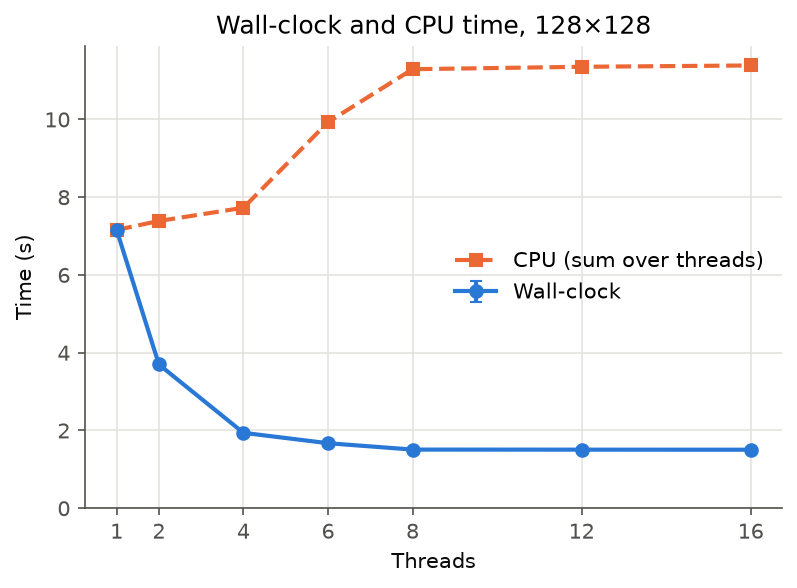
\includegraphics[width=\linewidth]{cpu_time.png}
    \caption{Wall-clock time and CPU time (sum over threads) on the $128\x128$ image.}
    \label{fig:cputime}
\end{figure}

\subsection{Effect of the bandwidth}
\label{sec:bandwidth}
Table~\ref{tab:bandwidth} and Figure~\ref{fig:bandwidth} show the effect of $h$ on the $96\x96$
image. A larger bandwidth smooths the density: the number of clusters falls from 75 to 3 and the
iterations needed to converge from 75 to 19, so both versions get faster.
Figure~\ref{fig:segmentations} shows the visual effect: $h \approx 12$ separates the main objects,
while $h = 24$ already merges, for example, the boat and the sea.

\begin{table}[!htb]
\centering
\small
\begin{tabular}{@{}rrrccr@{}}
\toprule
$h$ & $K$ & iter & seq (s) & par (s) & $S_{tot}$ \\ \midrule
6  & 75 & 74.9 & 5.530 & 0.850 & $6.5\x$ \\
8  & 30 & 61.9 & 5.118 & 0.704 & $7.3\x$ \\
12 & 6  & 42.9 & 4.265 & 0.499 & $8.5\x$ \\
16 & 5  & 30.5 & 3.499 & 0.360 & $9.7\x$ \\
24 & 4  & 23.2 & 3.329 & 0.279 & $11.9\x$ \\
32 & 3  & 18.6 & 3.463 & 0.228 & $15.2\x$ \\ \bottomrule
\end{tabular}
\caption{Effect of the bandwidth ($96\x96$, \texttt{par} with 8 threads). $K$: clusters;
iter: mean iterations per point.}
\label{tab:bandwidth}
\end{table}

The speedup grows with $h$, from $6.5\x$ to $15.2\x$. Dividing the time by the iterations explains
why: the cost of one iteration of \texttt{par} is constant ($11.3$\,ms at $h=6$, $12.3$\,ms at
$h=32$), because the vector loop always evaluates all the neighbours, while the cost of one
iteration of \texttt{seq} grows from 74\,ms to 186\,ms, because with a larger $h$ fewer neighbours
fall beyond the cutoff and fewer exponentials are skipped. The speedups above $8\x$ are therefore
not superlinear thread scaling: they come from comparing a vector loop with a fixed cost against a
scalar baseline whose cost depends on $h$. For the same reason the SIMD gain is smaller at small
$h$.

\subsection{Effect of the scheduling policy}
\label{sec:schedule}
Figure~\ref{fig:schedule} compares the OpenMP schedules with 8 threads. Plain \texttt{static} is
the slowest (2.24\,s, $+42\%$ over the best): it gives each thread one contiguous block of $N/8$
pixels, i.e.\ one horizontal band of the image, and the number of iterations depends on the region
(uniform sky converges quickly, textured areas slowly), so some threads finish much later than
others. \texttt{static,1} distributes the pixels in round-robin and is already as good as the dynamic
policies (1.60\,s), which shows that the imbalance comes from the spatial correlation of the work.
All the other policies are within 5\% of each other (1.58--1.65\,s); \texttt{dynamic,1} has the
largest variance. We use \texttt{dynamic,16}, which balances the load with a modest number of
dispatches.

\begin{figure}[!htb]
    \centering
    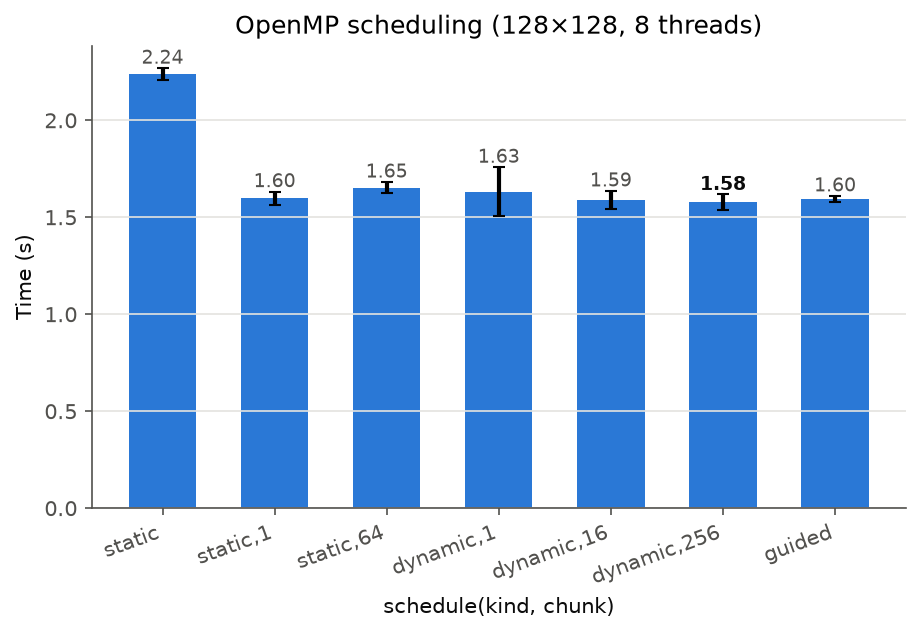
\includegraphics[width=\linewidth]{schedule.png}
    \caption{Time with different OpenMP scheduling policies ($128\x128$, 8 threads, 95\% CI). The
    best one is in bold.}
    \label{fig:schedule}
\end{figure}

\subsection{Effect of the memory layout}
Figure~\ref{fig:layout} compares the SoA and AoS layouts with the same vectorized loop. SoA is
faster by 7.7\% on one thread (7.18 vs 7.73\,s) and by 8.3\% on 8 threads (1.51 vs 1.64\,s). The
difference is small because the working set ($16\,384 \x 12$\,B $= 192$\,KB per layout) fits in
the L2 cache and the loop is compute-bound; with AoS the cost is the extra de-interleaving of the
stride-3 loads, not memory bandwidth.

\begin{figure}[!htb]
    \centering
    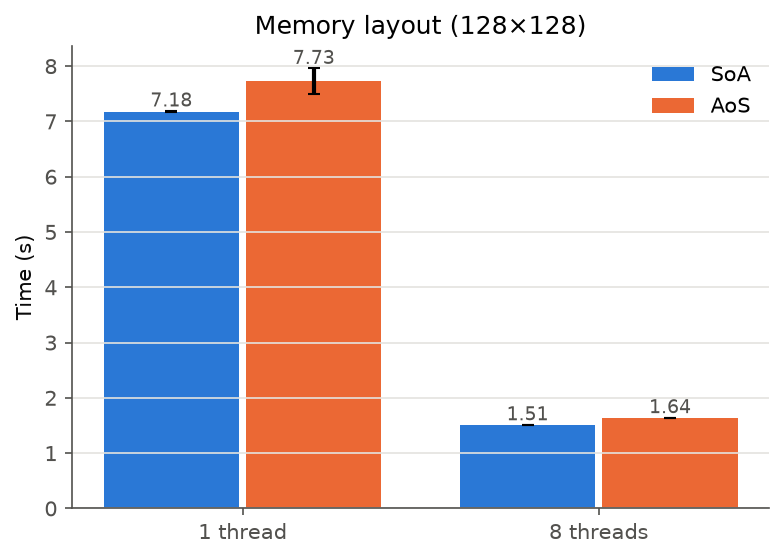
\includegraphics[width=0.85\linewidth]{layout.png}
    \caption{SoA vs AoS layout ($128\x128$, \texttt{par}, 95\% CI).}
    \label{fig:layout}
\end{figure}

\subsection{Bottleneck analysis}
\begin{itemize}
    \item \textbf{Compute, not memory}: the dataset fits in cache and is only read; one kernel
    evaluation costs $\approx 0.63$\,ns on one P-core with SIMD ($7.16\,\text{s} / 1.14\cdot10^{10}$
    evaluations). The exponential dominates the arithmetic of the loop.
    \item \textbf{Heterogeneous cores}: beyond 4 threads the speedup is limited by the slow
    E-cores, not by the algorithm.
    \item \textbf{Wasted work in SIMD}: the branchless cutoff computes the kernel also for the far
    neighbours, which limits the vector gain to $1.84\x$ at $h = 12$.
\end{itemize}

\section{Discussion}

\paragraph{Amdahl's law.} The sequential fraction of the parallel program is mode detection
(0.15\,ms over 7.16\,s, $f \approx 2\cdot10^{-5}$). By Amdahl's law~\cite{amdahl1967} this would
allow a speedup close to $p$ on any realistic number of cores, so the sequential part is not what
limits the scaling. The real limit is the hardware: the 8 cores are not equal, and the ideal
speedup is about 5 P-core equivalents, not 8.

\paragraph{Gustafson's law.} The work per point grows with $N$, so with larger images the parallel
fraction becomes even more dominant~\cite{gustafson1988}. Our sizes already show this: efficiency
is the same from $64^2$ to $128^2$ because the overhead is negligible even at the smallest size.
A weak-scaling experiment was not run because $O(N^2)$ work makes it impossible to keep the work
per thread constant without very large images.

\paragraph{Overheads.} Thread creation and scheduling cost microseconds, against more than 0.1\,s of
work; oversubscription (12--16 threads) does not change the time. The overhead visible in the CPU
time comes from the slower E-cores, not from OpenMP.

\paragraph{Limitations.}
\begin{itemize}
    \item The laptop has no fan: under continuous load at 8 threads the time grows from 1.55 to
    1.85\,s in 20\,s and by about 50\% after 2 minutes. The cool-down between runs mitigates it,
    but the absolute times still depend on the temperature.
    \item macOS does not allow fixing the CPU frequency or pinning threads to cores, so the
    placement of threads on P/E cores is decided by the operating system.
    \item Because of the $O(N^2)$ cost, the images are small ($\le 128^2$ pixels); full-resolution
    images would need an approximate neighbour search.
\end{itemize}

\paragraph{Lessons learned.} Vectorization needs the whole loop body to be inline and branchless:
a single library call (\texttt{std::exp}) was enough to cancel it. A fair baseline must use the
same arithmetic as the optimized versions, otherwise the measured speedup mixes different
algorithms. On heterogeneous CPUs, the speedup should be read against the real capacity of the
cores, not against the number of threads.

\section{Conclusions}
We implemented mean shift clustering for colour image segmentation in C++ with OpenMP and SIMD.
The parallelization needs no synchronization other than reductions, and the results are validated
against the sequential baseline: identical clusters and labels, modes within 0.08 on the 0--255
scale.

The best configuration is the \texttt{par} variant with SoA layout, 8 threads and dynamic
scheduling (\texttt{dynamic,16}): on a $128\x128$ image with $h = 12$ it runs in 1.51\,s against
13.15\,s of the scalar baseline, a speedup of $8.72\x$ ($1.84\x$ from vectorization, $4.75\x$ from
threads), and up to $15.2\x$ for large bandwidths. Thread scaling is almost linear on the 4
performance cores and saturates on the efficiency cores.

Future developments: skipping the far neighbours also in the vector loop (e.g.\ sorting or
bucketing the points by colour, or a k-d tree), the blurring variant of mean shift which converges
in fewer iterations, adding the spatial coordinates to the feature space (joint spatial-range
mean shift~\cite{comaniciu2002}), and a GPU implementation for full-resolution images.

{\small
\bibliographystyle{ieee}
\bibliography{refs}
}

\section*{Appendix}
\begin{enumerate}
\item \textbf{Computer Vision components:} the project implements mean shift, a non-parametric
feature-space analysis technique used for mode seeking and image segmentation. The algorithm
performs kernel density estimation and gradient ascent on pixel colour coordinates (RGB).
\item \textbf{Contributions:}
	\begin{enumerate}
	\item \textbf{Ideas:} identified the independence of the points and the use of dynamic
	scheduling for the irregular workload.
	\item \textbf{Formulations:} reformulated the Gaussian weighting with a branchless cutoff and an
	inline exponential to allow SIMD processing.
	\item \textbf{Software/Coding:} implemented the whole C++ codebase (sequential baseline, SIMD,
	OpenMP and layout variants), the benchmark harness and the Python scripts for preprocessing and
	plots.
	\item \textbf{Experiments:} designed the benchmark protocol (warm-up, repetitions, confidence
	intervals, cool-down) and the experiments on threads, bandwidth, scheduling and layout on
	BSDS500 images.
	\item \textbf{Analysis:} performed the speedup, efficiency and bottleneck analysis.
	\end{enumerate}
\item \textbf{Authorship:} I confirm that I am the sole author of this writeup and the associated code.
\end{enumerate}

\end{document}
